% !Mode:: "TeX:UTF-8"
\documentclass[QAofGroup.tex]{subfiles}

\begin{document}
%-=-=-=-=-=-=-=-=-=-=-=-=-=-=-=-=-=-=-=-=-=-=-=-=
%
%	CHAPTER
%
%-=-=-=-=-=-=-=-=-=-=-=-=-=-=-=-=-=-=-=-=-=-=-=-=

%%================================================================
\chapter{20171103}\label{ch1103}
%----------------------------------------------------------------------------------------

\begin{qst}\label{Q2017110301}
我想把源码加进appendix里面,双栏,请问有没人能指导一下?\index{源码双栏}
\end{qst}
\ans fancyvrb package 或者minipage。
参见\url{https://tex.stackexchange.com/questions/321750/listing-source-code-in-two-columns}

\begin{qst}\label{Q2017110302}
有人帮忙看看红色框内的文字是怎么平白无故出来的吗?\index{随机文本}

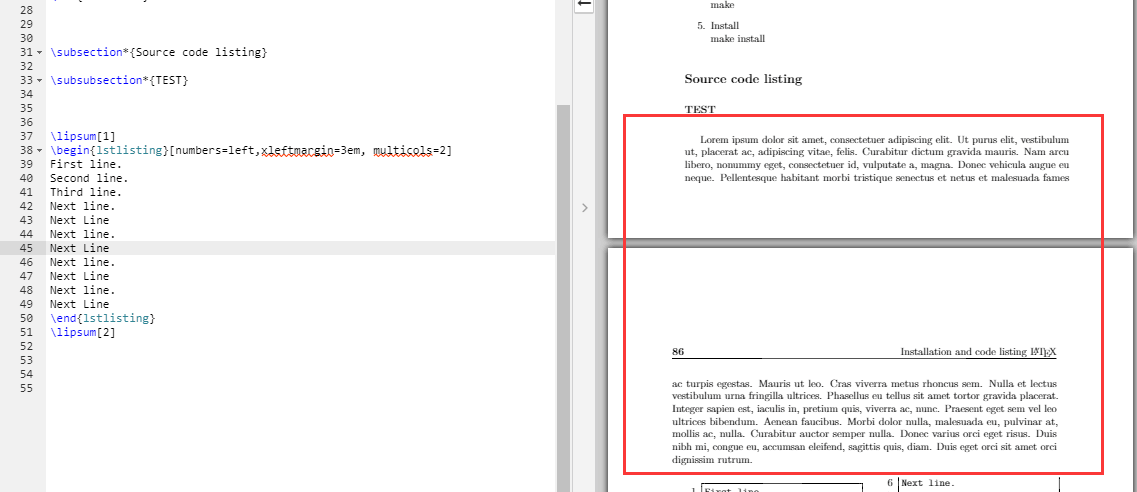
\includegraphics[width=0.65\textwidth]{pic08.png}
\end{qst}
\ans 你不是写了lipsum么,它是用来生成随机文本的。

\begin{qst}\label{Q2017110303}
直角标记怎么标记?\index{直角标记}

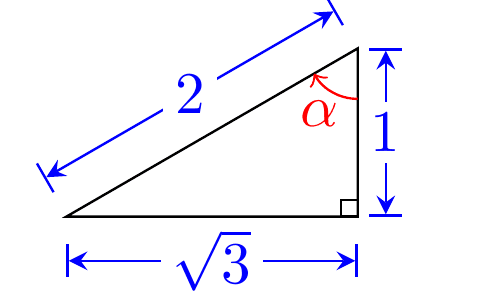
\includegraphics[width=0.45\textwidth]{pic09.png}
\end{qst}
\ans
\begin{verbatim}
\newcommand{\chuizhi}[2]
 {\draw[thick,red]($ (#1)!0.15!(#2) $)
  coordinate(c1)--($ (c1)!1!-90:(#1) $)coordinate(c2)--($ (c2)!1!-90:(c1) $);}
\begin{tikzpicture}
%画直角坐标系
\draw[thick,-latex](-3,0)--(3,0)node[below]{$ x $};
\draw[thick,-latex](0,-3)--(0,3)node[left]{$ y $};
%画椭圆
\draw[thick,blue](2,0)arc(0:360:2 and 1.732);
%定义坐标
\coordinate[label=above:$ P $](P)at(2*cos 60,1.732*sin 60);
\coordinate[label=below:$ F_1 $](f1)at(-1,0);
\coordinate[label=below:$ F_2 $](f2)at(1,0);
\coordinate[label=225:$ B $](B)at(-2,0);
\coordinate[label=-45:$ A $](A)at(2,0);
\coordinate[label=45:$ N $](N)at(0,2);
\coordinate[label=35:$ H $](H)at($ (N)!(f2)!(P) $);
%找交点
\tkzInterLL(f1,P)(f2,H) \tkzGetPoint{G}
\coordinate[label=45:$ G $](g)at(G);
%画切线
\draw[thick,blue,domain=-1:3]plot(\x,{2-(1/2)*\x});
%连线
\draw[thick,blue](B)--(H)(f1)--(g)(f2)--(g)(A)--(H)(f2)--(P);
\draw[thick,blue,dashed](0,0)--(H);
%标记原点
\node at (-.2,-.2){$ O $};
%画直角符号
\chuizhi{H}{g}
%\draw[thick,red]($ (H)!0.15!(g) $)
coordinate(c1)--($ (c1)!1!-90:(H) $)coordinate(c2)--($ (c2)!1!-90:(c1) $);
%画点
\foreach \x in {P,f1,f2,B,A,N,H,g}
\shade[ball color=red](\x)circle(1.3pt);
\end{tikzpicture}
\end{verbatim}
\newcommand{\chuizhi}[2]{\draw[thick,red]($ (#1)!0.15!(#2) $)coordinate(c1)--($ (c1)!1!-90:(#1) $)coordinate(c2)--($ (c2)!1!-90:(c1) $);}
\begin{tikzpicture}
%画直角坐标系
\draw[thick,-latex](-3,0)--(3,0)node[below]{$ x $};
\draw[thick,-latex](0,-3)--(0,3)node[left]{$ y $};
%画椭圆
\draw[thick,blue](2,0)arc(0:360:2 and 1.732);
%定义坐标
\coordinate[label=above:$ P $](P)at(2*cos 60,1.732*sin 60);
\coordinate[label=below:$ F_1 $](f1)at(-1,0);
\coordinate[label=below:$ F_2 $](f2)at(1,0);
\coordinate[label=225:$ B $](B)at(-2,0);
\coordinate[label=-45:$ A $](A)at(2,0);
\coordinate[label=45:$ N $](N)at(0,2);
\coordinate[label=35:$ H $](H)at($ (N)!(f2)!(P) $);
%找交点
\tkzInterLL(f1,P)(f2,H) \tkzGetPoint{G}
\coordinate[label=45:$ G $](g)at(G);
%画切线
\draw[thick,blue,domain=-1:3]plot(\x,{2-(1/2)*\x});
%连线
\draw[thick,blue](B)--(H)(f1)--(g)(f2)--(g)(A)--(H)(f2)--(P);
\draw[thick,blue,dashed](0,0)--(H);
%标记原点
\node at (-.2,-.2){$ O $};
%画直角符号
\chuizhi{H}{g}
%\draw[thick,red]($ (H)!0.15!(g) $)coordinate(c1)--($ (c1)!1!-90:(H) $)coordinate(c2)--($ (c2)!1!-90:(c1) $);
%画点
\foreach \x in {P,f1,f2,B,A,N,H,g}
\shade[ball color=red](\x)circle(1.3pt);
\end{tikzpicture}

\begin{qst}\label{Q2017110304}
Asymptote画图怎么插入tex里?还是只能插图片,不能插代码?\index{Asymptote插图}
\end{qst}
\ans
\begin{verbatim}
\usepackage{asymptote}
\begin{document}
\begin{asy}
asymptote 代码写这里
\end{asy}
\end{document}
\end{verbatim}
可是必须先 pdflatex,再执行 asymptote,再执行 pdflatex。
建议先生成 pdf再插入,方便调试。
尤其当你的 tex文件很大的时候,比如是一本书,为了调试个图片代码,不得不把整本书编译一下……

\begin{qst}\label{Q2017110305}
align*环境上下的空隙怎么调啊?上面倒是好了,下面的还是太大。
\index{公式与上下文的间距}
\end{qst}
\ans 可以修改\LaTeX{}预定义的垂直间距命令的值来调整。

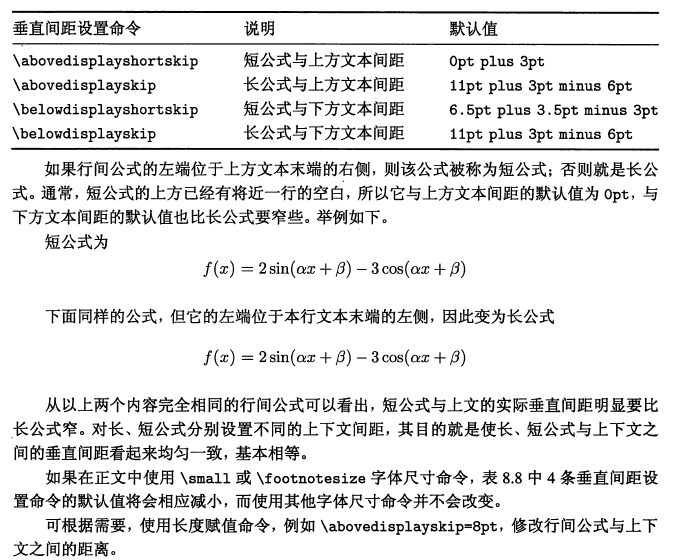
\includegraphics[width=0.65\textwidth]{pic10.png}

\begin{qst}\label{Q2017110306}
 有没有推荐适合tex的编辑器 winedt 10好像破解比较麻烦。\index{编辑器的选择}
\end{qst}
\ans 买一下,一百来块钱。其他可选的很多。还有啊,这种问题,网上的专业的回答一大把,专门列出了各个编辑器的特点,比如这里\url{https://www.zhihu.com/question/19954023?rf=29771547}为什么不自己看一看呢?还有这里 \url{https://en.wikipedia.org/wiki/Comparison_of_TeX_editors} 你听过的没听过的编辑器都在这里。
 
\begin{qst}\label{Q2017110307}
有没有好看的数学试卷模板分享阿,要给学校学生出期中考试试卷了。\index{试卷模版}
\end{qst}
\ans 可以参考这个\url{http://blog.sciencenet.cn/blog-292361-1022766.html}。

\begin{qst}\label{Q2017110308}
求问beamer中段首缩进怎么弄,我在导言区加了\\
\verb|\usepackage{indentfirst}|\\
 还是没用。
\end{qst}
\ans 试试这个\verb|\setlength{\parindent}{1em}|。


\begin{qst}\label{Q2017110309}
beamer中怎么设置让每行的最后一个单词断开呀?感觉行末没有对齐好难受。\index{beamer分散对齐}
\end{qst}
\ans 左对齐那是beamer的默认格式啊,可以用在导言区加如下语句\\
 \mintinline{tex}{\usepackage{ragged2e}}\\
 \mintinline{tex}{\justifying\let\raggedright\justifying}\\
 来实现分散对齐,也就是你说的两端对齐。
 另外,用babel,可以自动断词。
 
\begin{qst}\label{Q2017110310}
	如何在pdf文档中显示代码及其结果。\index{显示代码及结果}
\end{qst}
\ans 使用codeshow宏包的codeshow环境。
%\begin{codeshow}
%	\LaTeX{} is a 惊喜。
%\end{codeshow}
%\begin{codeshow}
%	\[
%	 \sin^2x+\cos^2x=1
%	\]
%\end{codeshow}
\end{document} 